\documentclass{article}
\usepackage{charter}
\usepackage[margin=1in]{geometry}
\usepackage{fancyhdr,graphicx}
\usepackage{xspace}

\fancypagestyle{firstpage}{%
  \fancyhf{} % Clear header/footer
  \renewcommand{\headrulewidth}{0pt}%
  \renewcommand{\footrulewidth}{1pt}%
  % Add more detail here if needed
}
\fancypagestyle{otherpages}{%
  \fancyhf{}% Clear header/footer
  \renewcommand{\headrulewidth}{1pt}%
  \renewcommand{\footrulewidth}{1pt}%
  % Add more detail here if needed
}

\AtBeginDocument{\thispagestyle{firstpage}}
\pagestyle{otherpages}

\setlength{\parindent}{0pt}
\setlength{\parskip}{1ex}

\begin{document}

\vspace*{\dimexpr-\headsep-\headheight-1pt}

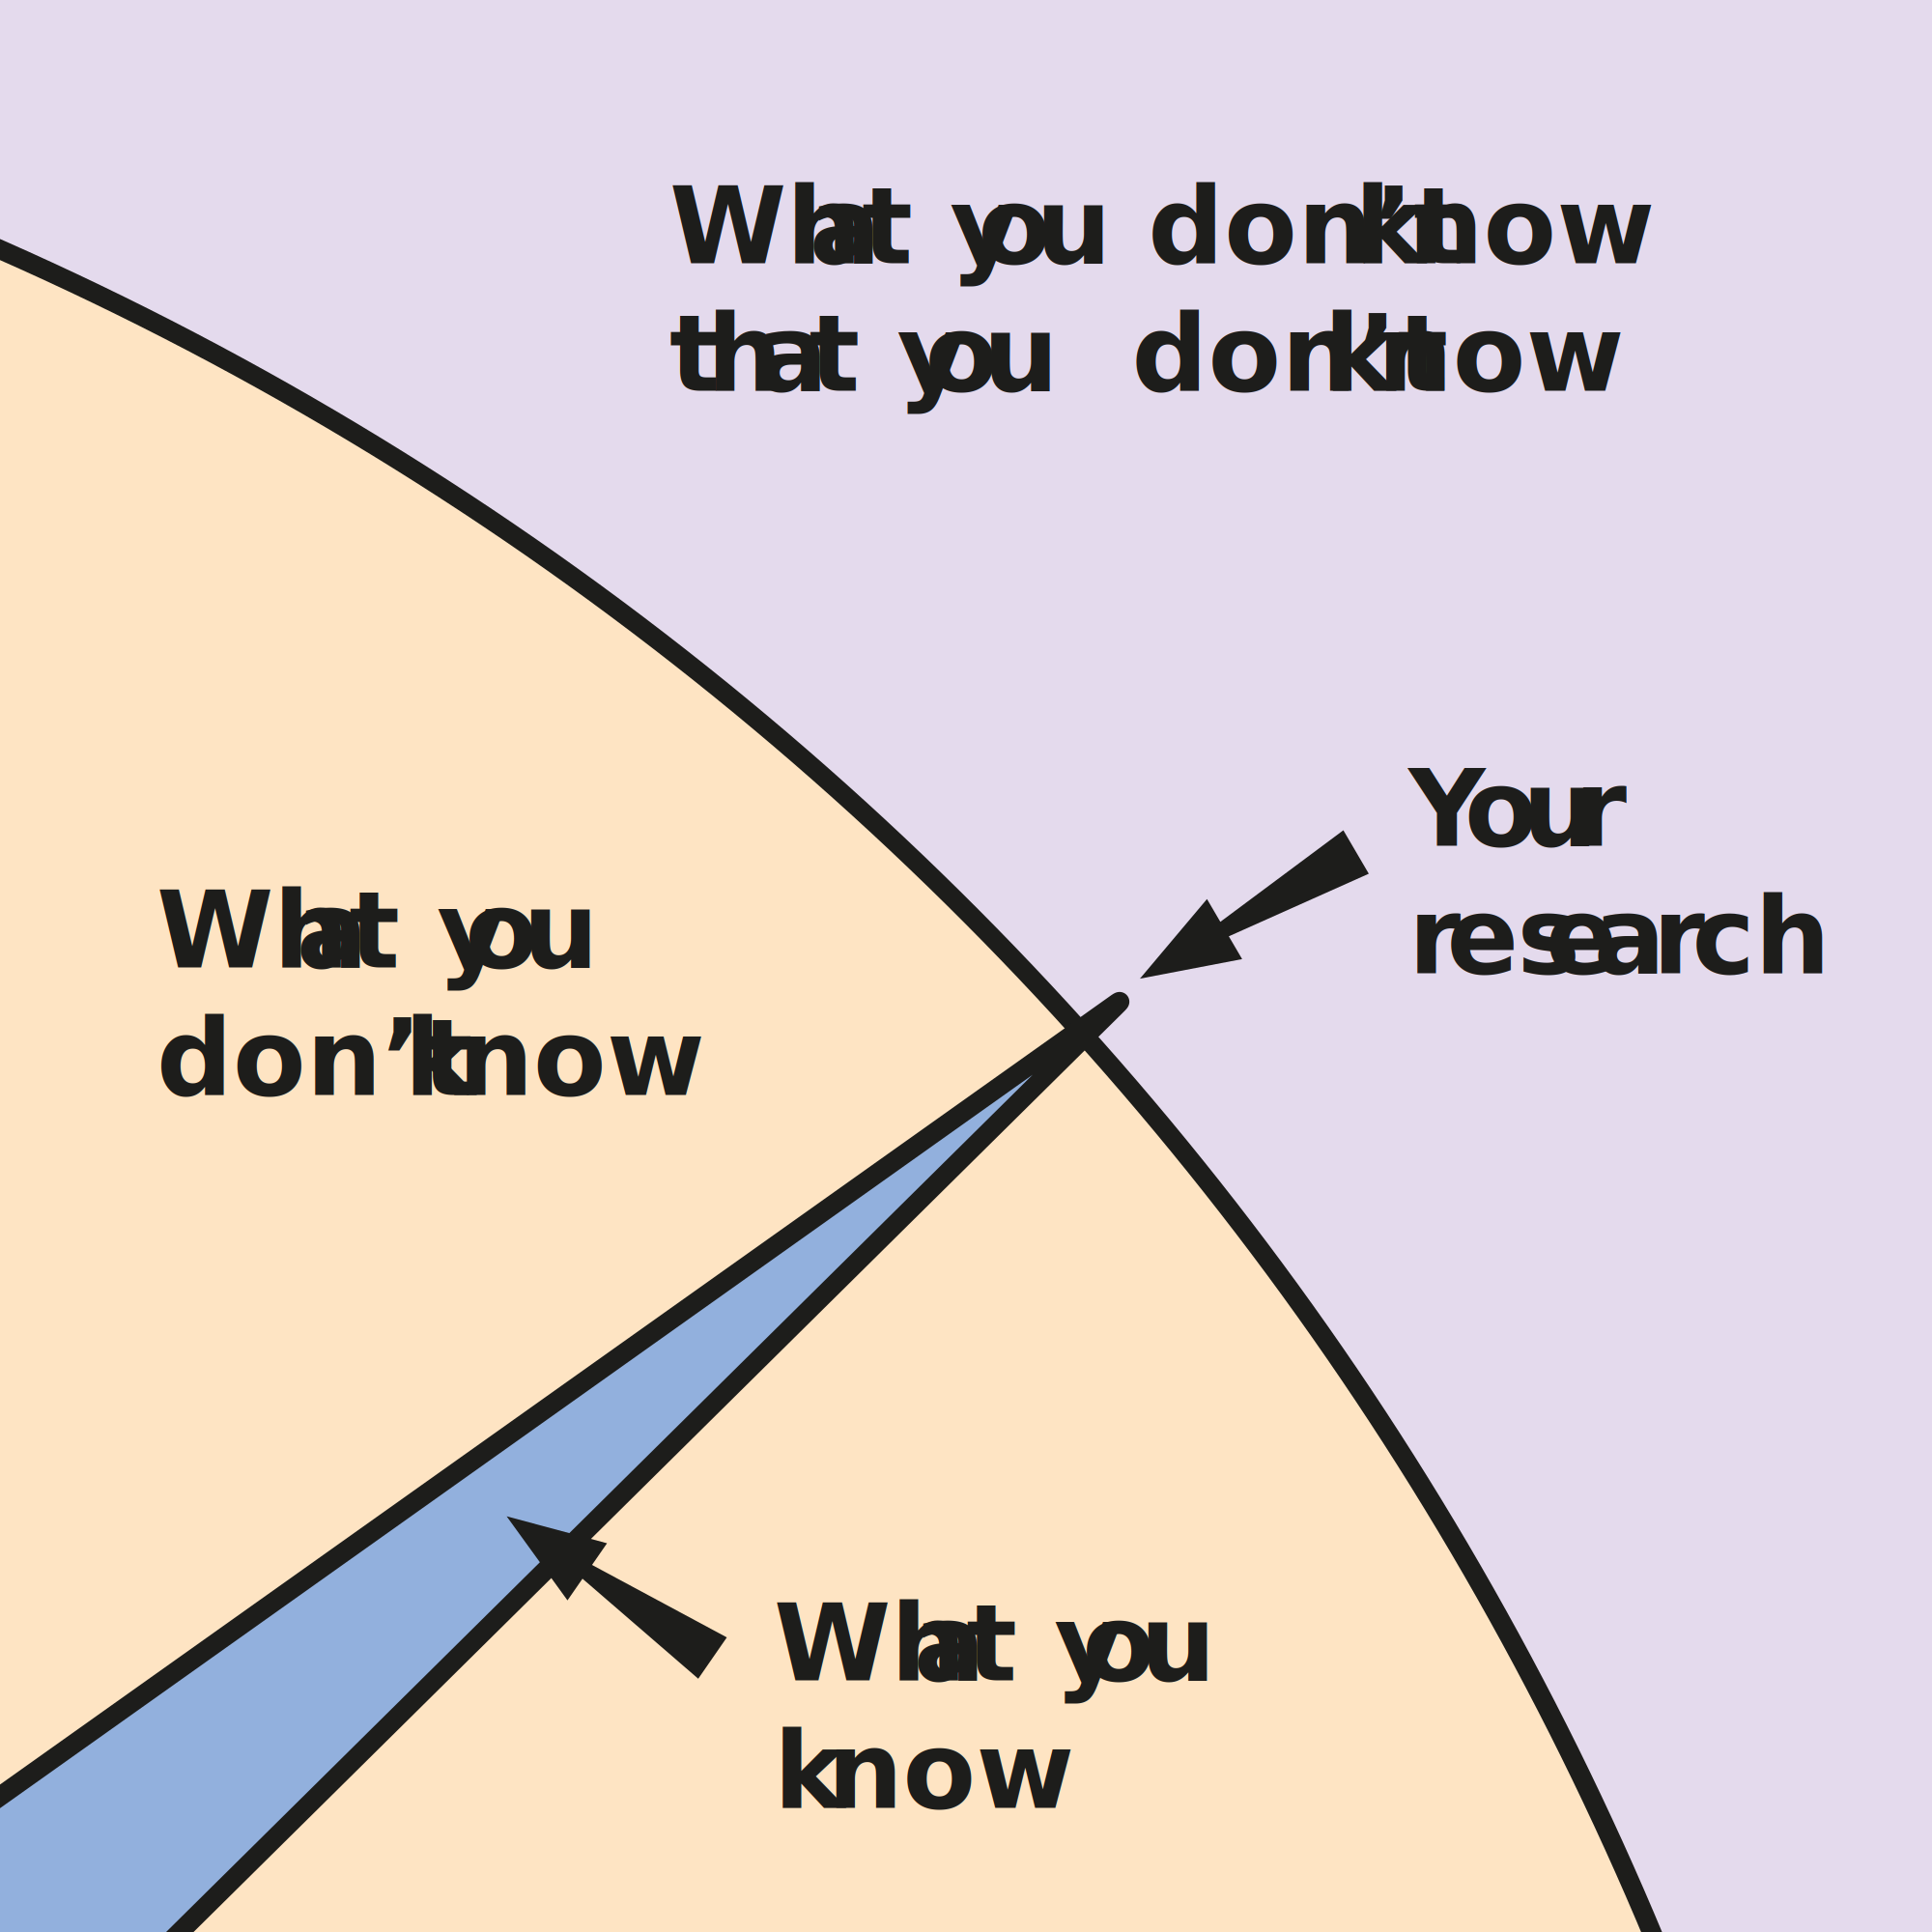
\includegraphics[width=1in]{logo.jpg}

\rule{\linewidth}{1pt}

\bigskip


%----------------------------------------------------------------------------------------
%	YOU ONLY NEED TO FILL IN THE FOLLOWING LATEX MACROS
%----------------------------------------------------------------------------------------

% Title of the paper
\newcommand{\PaperTitle}{Paper's Title\xspace}

% Full name of the authors
\newcommand{\AuthorOne}{Author \#1\xspace}
\newcommand{\AuthorTwo}{Author \#2\xspace}
\newcommand{\AuthorThree}{Author \#3\xspace}
\newcommand{\AuthorFour}{Author \#4\xspace}

% Institution
\newcommand{\Institution}{Institution of the Authors\xspace}
\newcommand{\InstitutionAddress}{Institution Address\xspace}
\newcommand{\City}{City\xspace}
\newcommand{\Country}{Country\xspace}

% Full name of the Journal's Editor in Chief
\newcommand{\EditorInChief}{Name of Editor in Chief\xspace}

% Journal
\newcommand{\Journal}{Name of the Journal\xspace}

% Body
\newcommand{\Contribution}{X\xspace}
\newcommand{\Problem}{Y\xspace}
\newcommand{\Solution}{Z\xspace}
\newcommand{\Evaluation}{D\xspace}
\newcommand{\NoveltyClaim}{E\xspace}

% List of contributions
\newcommand{\ContributionOne}{Contribution A.\xspace}
\newcommand{\ContributionTwo}{Contribution B.\xspace}
\newcommand{\ContributionThree}{Contribution C.\xspace}
\newcommand{\ContributionFour}{Contribution D.\xspace}

% Suggested editors
\newcommand{\EditorOne}{Editor \#1\xspace}
\newcommand{\EditorOneExpertise}{A\xspace}

\newcommand{\EditorTwo}{Editor \#2\xspace}
\newcommand{\EditorTwoExpertise}{B\xspace}

\newcommand{\EditorThree}{Editor \#3\xspace}
\newcommand{\EditorThreeExpertise}{C\xspace}

%----------------------------------------------------------------------------------------
%	YOUR NAME AND CONTACT INFORMATION
%----------------------------------------------------------------------------------------

\hfill
\begin{tabular}{ l @{} }
  \today \\[12pt] % Date
  \Institution\\
  \InstitutionAddress\\
  \City, \Country
\end{tabular}


%----------------------------------------------------------------------------------------
%	LETTER CONTENT
%----------------------------------------------------------------------------------------

\bigskip

Dear \EditorInChief,\\Editor-in-Chief of \textit{\Journal}

\bigskip

We wish to submit the research manuscript entitled ``\PaperTitle,” by \AuthorOne, \AuthorTwo, \AuthorThree, and \AuthorFour. We certify that all the authors participated in the preparation of this manuscript and agree with its submission. This manuscript has not been published elsewhere and is not under consideration by another journal.

This work contributes to the state-of-the-art of \Contribution.
We propose a novel approach to \Problem based on \Solution.
We evaluate our approach on \Evaluation.
Furthermore, we provide the first investigation on \NoveltyClaim.

In summary, our contributions are the following:

\begin{itemize}
	\item \ContributionOne
    \item \ContributionTwo
	\item \ContributionThree
	\item \ContributionFour
\end{itemize}

We would like to suggest the following editors to handle this submission, based on their expertise:

\begin{itemize}
    \item \EditorOne, for his strong knowledge of \EditorOneExpertise.
    \item \EditorTwo, for her contributions to \EditorTwoExpertise.
    \item \EditorThree, for her expertise in \EditorThreeExpertise.
\end{itemize}

Please do not hesitate to contact us in case you require further information regarding this manuscript.

\bigskip

Sincerely yours,

\vspace{50pt}

\AuthorOne\\ \\On behalf of \AuthorTwo, \AuthorThree, and \AuthorFour

\end{document}